\documentclass[letterpaper,twocolumn,11pt]{article}
\usepackage{usenix-2020-09}
\usepackage{graphicx}
\usepackage{amsmath}

% Report due date
\date{December 16, 2022}

% Project Title
\title{%
  {\Large \bf An Interactive Visualizer for Equality Solvers using E-Graphs}\\%
  {\large Princeton University COS 516 Course Project (Fall '22)}%
}

%for single author (just remove % characters)
\author{ {\rm Ryan Torok}\\ Princeton University \and {\rm Leon Sch\"urmann}\\ Princeton University
% copy the following lines to add more authors \and {\rm Name}\\
%Name Institution
} % end author
\begin{document}

\maketitle

\section{Introduction}

The \textit{Theory of Equality} (TOE) is a theory in first-order logic which
axiomatizes that the equality operator (=) behaves reasonably\cite{bm}. A
well-known algorithm for finding all equivalence classes of a given formula,
which constitutes a theory solver for TOE, is to list all terms that appear in
the formula, then iterate through pairs of terms, adding terms to equivalence
classes using a union-find data structure by repeatedly applying the rule $a = b
\rightarrow f(a) = f(b)$, where $a$ and $b$ are terms, and $f$ is a function
symbol. In the worst case, running this procedure until no more matches are
possible requires quadratic time. While this is still a polynomial-time
algorithm, it is rather naive in its method to choose new pairs and it is
definitely possible to do better.

E-graphs \cite{egraphs} improve the time complexity of this procedure by
representing the terms of an expression as a directed acyclic graph (DAG), such
that constant or function symbols are represented using vertices, and the
composition of terms is given through the edges. Each vertex belongs to a given
\textit{equality class}, which defines subterms that are equivalent as per
equivalence under the TOE. Edges in this graph lead from a given vertex $v$,
parameterized by an argument index $0 \geq i < \text{arity}(v)$ towards an
equivalence class, which binds the symbol's $n$th parameter to any element of
this class. For example, Figure \ref{fig:egraph} represents an E-graph for the
formula $(a * 2) / 2$.

This structure is an inherently compact representation of possible alternate
expressions of a \textit{program} (defined as the top-level term in the provided
expression). This characteristic makes it possible to efficiently find all
equality classes without requiring the linear pass over all terms. In addition
to the equivalences established by the equivalence operator as axiomatized by
the TOE in first-order logic with equality, E-graphs can set additional
expressions equal by a user-provided, arbitrary set of additional rewrite rules
(unidirectional definitions of allowed term transformations). This makes
E-graphs a powerful tool for many applications such as optimizing compilers,
where there are a varity of ways to express and equivalent concept. Given that
E-graphs can encompass a multitude of equivalent programs, this enables
compilers to search them for expressions which are ideal under a set of
constraints, for instance in an effort to eliminate common sub-expressions. This
particular application area of E-graphs is called \textit{equality saturation}.

\texttt{egg} is a popular Rust library that implements E-graphs, and has seen
widespread use in the research community, which can be attributed to its
flexibility, efficiency and ergonomic developer interface \cite{egg}.

\begin{figure}[t]
    \centering
    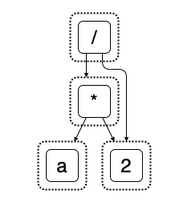
\includegraphics[width=.5\columnwidth]{egraph.png}
    \caption{E-graph representing the formula $(a * 2) / 2$ \cite{egg}}
    \label{fig:egraph}
\end{figure}

Unfortunately, the precise mechanisms employed both within the congruence
closure algorithm, as well as the extended e-graph data structures, can be
unintuitive for novice users. We presume that an interactive visualization can
help demonstrate the basic concepts behind reasoning about equality under a
given set of rewrite rules. In this project, we create \texttt{eggviz}, a
web-based visualization tool that allows the user to interactively explore the
equivalence-matching procedure and program optimization techniques in a
step-by-step manner.

\section{User Interface Overview}

We begin by providing a high-level overview over the feature-set and ideas
incorporated into \texttt{eggviz}. Its user interface follows a layout inspired
by the CDCL solver as introduced in the
course\footnote{\url{https://www.cs.princeton.edu/courses/archive/fall22/cos516/cdcl/}}.
Figure \ref{fig:my_label} contains a screenshot providing a high-level overview
of the main \texttt{eggviz} user interface components. In its top-bar, a user
can enter a program following a LISP-inspired syntax. We choose this syntax as
it is easy to parse (including implementing full syntax error handling) and
simple for the user to reason about its equivalent E-graph. We define our LISP
syntax formally in Section \ref{sec:lispylang}.

Through the application's left-hand control pane, the user can add
\textit{rewrite rules} to be applied to the program, using the same LISP-like
syntax as defined in \ref{sec:lispylang}. Following adding a program and at
least one rewrite rule, the user can press the \texttt{Graph!} button to show an
E-graph representation of the program. The graph, which we render through the
vis.js\cite{vis} library, represents each equivalence class (E-class) using a
different color. Unfortunately, vis.js does not support a grouping a set of
vertices into a class, as would be particularly useful to illustrate the concept
of equivalence classes. While extending vis.js to support such a visualization
mode is outside of the scope of this project, this could be a particularly
useful future task. We work around this limitation by introducing two distinct
types of nodes: \textit{box-shaped nodes}, which represent individual terms and
\textit{circular nodes}, which serve as a root node for each equivalence class.
Along with this distinction, we further establish two types of relations,
modeled through edges: terms in an equivalence class are connected by bold edges
without arrows to the root node of that class. The thinner, directed edges point
from a box-shaped node to a root node of the equivalence class of the subterm(s)
of the corresponding expression. These types of edges are also marked with a
number to correspond to the argument index of that subterm within the parent
term.

\texttt{eggviz} supports two usage modes: first, clicking on a rewrite rule at
the left pane will apply that rewrite rule iteratively until it can no longer be
applied. For this feature, it is up to the user to decide in what order to apply
the rewrite rules to generate the desired equivalences. The second mode of user
interaction is automatically applying all rewrite rules once, by clicking the
\texttt{Auto} button. This has the same effect as clicking all of the rewrite
rules in order. In other words, for a program with two rewrite rules $R_1$ and
$R_2$, \texttt{eggviz} would apply $R_1$ everywhere it can, then do the same
with $R_2$, but it will not return to $R_1$ afterwards, even if $R_2$ created
new instances where it could be applied (unless, of course, the user clicks
\texttt{Auto} or $R_1$ again).

\begin{figure*}
    \centering
    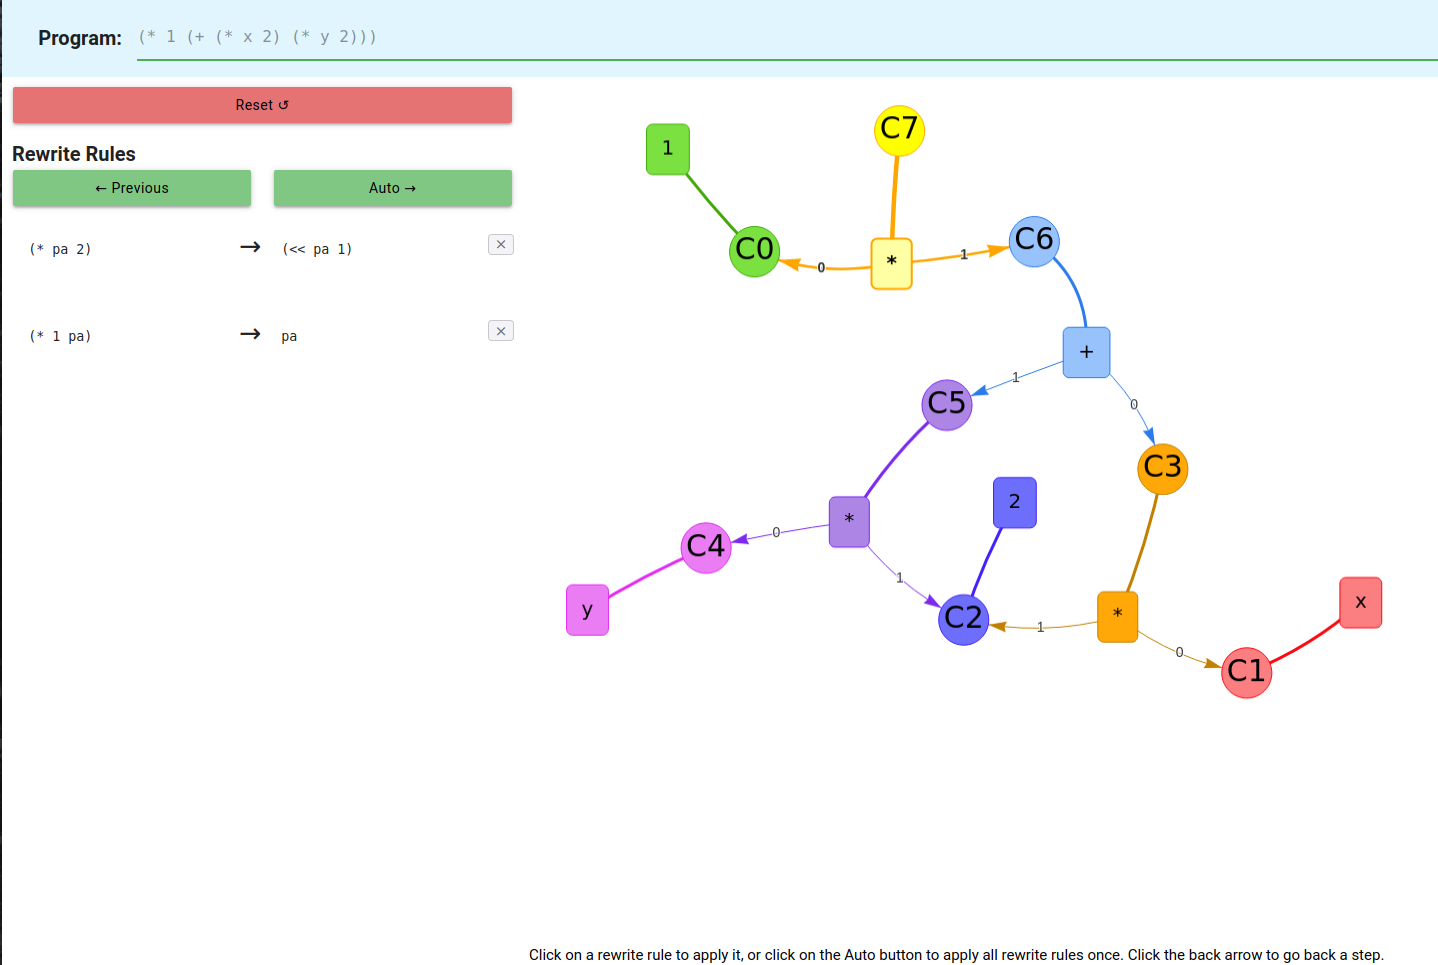
\includegraphics[width=\textwidth]{interface.png}
    \caption{The \texttt{eggviz} interface. The program is entered at the top,
      the rewrite rules at the left, and the graph is shown in the main display
      area.}
    \label{fig:my_label}
\end{figure*}

\section{Implementation and Internals}

\texttt{eggviz} is powered internally by \texttt{egg}, a Rust E-graph
library\cite{egg}. To integrate \texttt{egg} with \texttt{eggviz}, we implement
a parser for our LISP-like syntax, a dedicated \textit{single-step scheduler}
that allows the user to advance the state of the E-graph in a step-wise manner,
and a formatting mechanism for translating the graph state to JavaScript in a
Rust library which we import into our web page as a WebAssembly module. We also
implement and set of JavaScript functions responsible for taking the graph state
returned by Rust and drawing the graph for the user using vis.js. In this
section, we perform a deep dive on the design and implementation of each of
these features.

\subsection{LispyLang and Parsing}
\label{sec:lispylang}

LispyLang is the name we give to the LISP-like syntax we introduced in the
previous section and that \texttt{eggviz} uses for its program and rewrite
rules. LispyLang implements the following syntax:

\noindent
\begin{align*}
\text{Program} &: \text{Term} \\
\text{Term} &: \text{Symbol}\ |\ \text{(Symbol Term \ldots)} \\
\end{align*}

A \textit{Symbol} can be any string of characters that does not contain either
of the characters "\texttt{(}", "\texttt{ }", or \texttt{")"}. In other words,
all variables, numbers, and similar are all considered symbols, since neither
\texttt{eggviz} nor \texttt{egg} assume any particular arithmetic, so the symbol
\texttt{1} has no more inherent meaning than the symbol \texttt{x}. Likewise,
the behavior of function symbols is determined entirely through rewrite rules,
meaning the operator \texttt{+} could be defined to just produce the value 0
always or even take three arguments.

However, there are two rules \texttt{eggviz} does enforce with regard to
symbols: first, all applications of a symbol occurring across the program and
all rewrite rules must have the same \textit{arity}, or number of arguments. For
example, if a program included the term \texttt{(+ a b)}, then the terms
\texttt{(+ 1 2 3)}, \texttt{(+ 1)}, or \texttt{+} could not be used elsewhere in
the program or in any rewrite rule, since the $+$ operator was already declared
with an arity of 2.

Second, there is one type of symbol that is assigned special meaning:
\textit{generic variables}: By convention, these are any symbol beginning with
the character \texttt{p}. Generic variables are used to dictate that a rewrite
rule applies for all values of the generic variable. For example, the identity
property of the multiplication operator \texttt{*} can be written as the rewrite
rule \texttt{(* 1 pa) $\rightarrow$ pa}. This means that the symbol \texttt{*}
applied to the symbol \texttt{1} and any symbol can be rewritten as just that
symbol. The definition of generic variables is local to the rewrite rule in
which they appear. Likewise, to avoid confusion, variables beginning the
character \texttt{p} are not permitted within the program expression.

We designed LispyLang with a LISP-like syntax with prefix notation to aid
parsing and to make clear that no operator has any inherent meaning in the
system, including \texttt{*} and \texttt{+}. We implement a simple two-function
top-down parser for LispyLang that supports full handling of syntax errors
(which are written to the footer of the UI if they occur).

\subsection{Rewrites and the Single-Step Scheduler}

When the user indicates they want to graph a program, once the program and
rewrite rules are parsed and validated for syntax and pass the arity checker,
\texttt{eggviz} takes its internal representation of the program and rewrite
rules and produces a string with the syntax \texttt{egg} expects, which differs
from LispyLang only in its notation for generic variables. Next, \texttt{eggviz}
needs to respond to which rewrite rules the user chooses to apply.

Unfortunately, \texttt{egg} was not designed to be able to selectively apply a
single rewrite rule at at time; it only exposes an API to repeatedly apply all
rewrite rules until it can no longer find any new equality relations. At the
start of the project, we believed we would need to modify the \texttt{egg}
library in order to implement the interactivity we wanted for
\texttt{eggviz}. However, it turned out to be possible to allow selectively
applying rewrite rules using the unmodified \texttt{egg} library by using
(abusing?) one feature of \texttt{egg}'s API, the \textit{scheduler}.

The scheduler is a feature of \texttt{egg} intended to provide users control
over the precise equality saturation strategy used in \texttt{egg}'s iterations
over the E-graph. This is particularly useful given that there are combinations
of programs and rewrite rules for which, depending on the heuristic used to
determine which rewrites count as \textit{simplifying}, the simplification
process would never finish. For example, a bad simplification heuristic would
allow recursive rewrite rules like \texttt{pa}$\rightarrow$\texttt{(+ pa pa)} to
be applied forever. While \texttt{egg} can be provided \textit{limits} (such as
E-graph size and saturation time) at which it will terminate the equality
saturation process, the scheduler gives developers control of when which rewrite
rules will be applied and can, for instance, aid in early termination of the
equality search after a certain point in these runaway cases.

\texttt{egg} further allows passing a custom scheduler by implementing the
\texttt{Scheduler} trait, which we leverage for \texttt{eggviz} by implementing
the \texttt{SingleStepScheduler} type. Rather than just being intended to
prevent runaway rule applications, the single-step scheduler is designed to
selectively and iteratively apply rewrite rules based on the user's interaction
with \texttt{eggviz}. Specifically, it is programmed to take a rewrite rule and
apply only that rule for a single iteration, or, if the user clicks the Auto
button, apply all rules for a single iteration.

To achieve this, the single step scheduler, on the first iteration, tells
\texttt{egg} to apply only the rule(s) it wants to. For subsequent iterations,
the scheduler tells \texttt{egg} not to apply any rule. Then, because
\texttt{egg} decides to stop when the equality classes are unchanged by an
iteration, the process is halted after a single meaningful iteration followed by
a no-op. Our design of the single-step scheduler is the key piece enabling us to
transform what \texttt{egg} implements as an opaque one-shot process into a
step-wise procedure that grants the user a great deal of control and ability to
experiment with different rewrite rules. We also greatly generified the
scheduler and rewrite logic so that these components of the \texttt{eggviz}
library could be applied by future developers to a different language
implementation than LispyLang if desired.

\subsection{Wasm-JS Integration and Graphing}
Using the single-step scheduler, \texttt{eggviz} instructs \texttt{egg} to apply
exactly the rewrite rule(s) the user selects. This allows us to read the state
of the E-graph from \texttt{egg} after each transformation. This graph state is
transformed to a JavaScript object using a series of Maps that encode the
relationship between symbols, terms, and expressions.  Once we return the graph
state to JavaScript, we iterate over this map at multiple levels to draw the
graph.

Since E-graphs inherently store the function-argument relationship as an edge
between the function symbol and the e-class of the argument (rather than the
argument term), we designed our graph to have two types of nodes: one to serve
as the edge sink for each e-class, and the other to represent the terms in that
e-class. This separation of duty prevents a term whose argument is in an e-class
with a large number of members from needing to draw an edge to every member of
that e-class, making the graph very hard to read and understand.

One consequence of this design choice is that our displayed graph now has two
type of edges, one to represent arguments to a function symbol, and another to
connect terms within an e-class. We visually distinguish these two types of
edges by making the latter type much thicker and lack arrows. E-classes are also
visually represented by the color of their nodes. While we briefly considered a
basic \textit{color wheel} algorithm to produce contrasting colors, it was
eventually scrapped after we discovered that the vis.js library has a built-in
coloring feature that is much better at avoiding dark colors that would disguise
the text within the nodes.

\section{Example}

In this section, we provide a short example of how \texttt{eggviz}
functions. Figure \ref{fig:before} shows \texttt{eggviz}'s rendering of the
program \texttt{(* 1 (+ (* x 2) (* y 2)))}, with the rewrite rules \texttt{(* pa
  2) $\rightarrow$ (<< pa 1)} and \texttt{(* 1 pa) $\rightarrow$ pa}. These
rewrite intuitively correspond to the properties "1 times any number is itself"
and "any number times 2 is the same as left-shifting that number by one bit",
respectively.

Suppose we click on the second rewrite rule to apply it. This tells
\texttt{eggviz} to find any new equality relations based on the rule that "1
times any number is itself". In this case, this means that the entire program,
\texttt{(* 1 (+ (* x 2) (* y 2)))}, is equivalent to just the term \texttt{(+ (*
  x 2) (* y 2))}. In the E-graph, this corresponds to annotating the term rooted
at the outermost \texttt{*} operator with the same equality class as the term
rooted at the \texttt{+} operator. Figure \ref{fig:after_1} shows the change to
the graph that occurs after applying, this rewrite rule; namely, the outermost
\texttt{*} operator, originally part of its own equality class \texttt{C7}, was
merged into the equality class \texttt{C6}, which contains the \texttt{+} term.

Now, suppose we apply the first rewrite rule next. Figure \ref{fig:after_2}
shows the graph after applying this transformation. Two new terms are introduced
for \texttt{(<< x 1)} and \texttt{(y << 1)}, which are included in the same
equality classes as the terms \texttt{(* x 2)} and \texttt{(* y 2)},
respectively. Also, observe that the two \texttt{<<} nodes are the only new
nodes introduced to the graph at this step, since they could use the existing
\texttt{x} and \texttt{y} terms, respectively, and the symbol \texttt{1} from
the outermost \texttt{*} operator as their children.

\section{Implementation Breakdown}

Both of us contributed equally to this project. Here is a rough breakdown of who
worked on what:
\begin{itemize}
    \item Leon: Rewrite logic, single-step scheduler, language traits,
      WebAssembly API design, significant refactoring
    \item Ryan: UI controls and event handlers, LispyLang parser and error
      handling, \texttt{egg} library integration, graph beautification
    \item Pair-programmed: WebAssembly to JavaScript encoding conversion, vis.js
      library integration and graph display
\end{itemize}

Our implementation of \texttt{eggviz} is available on
GitHub\footnote{\url{https://github.com/lschuermann/eggviz}}, with a prebuilt
version deployed on GitHub
pages\footnote{\url{https://lschuermann.github.io/eggviz/}}. \texttt{eggviz} is
licensed under a AGPL-3.0 license and can be freely used, shared, modified and
inspected according to the terms of this license.

\bibliographystyle{plain}
\bibliography{report}

\begin{figure*}
    \centering
    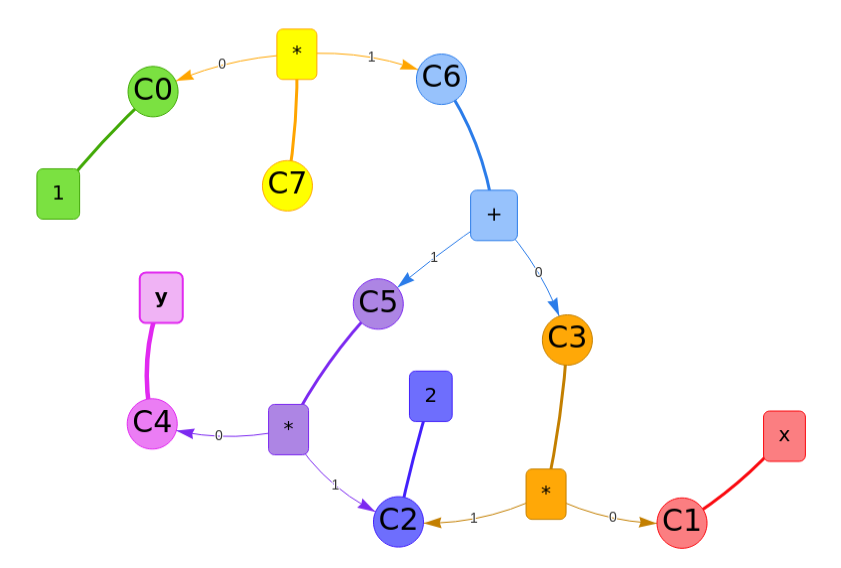
\includegraphics[width=1.2\columnwidth]{before.png}
    \caption{\texttt{eggviz} representation of the E-graph for the program
      \texttt{(* 1 (+ (* x 2) (* y 2)))}.}
    \label{fig:before}
\end{figure*}

\begin{figure*}
    \centering
    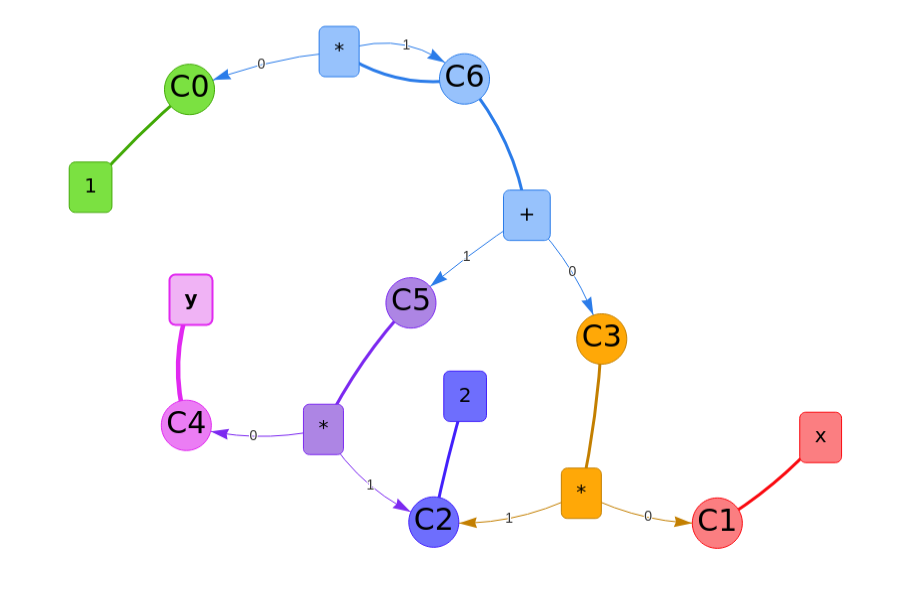
\includegraphics[width=1.2\columnwidth]{after-1.png}
    \caption{Graph from Figure \ref{fig:before} after applying the rewrite rule
      \texttt{(* 1 pa) $\rightarrow$ pa}. }
    \label{fig:after_1}
\end{figure*}

\begin{figure*}
    \centering
    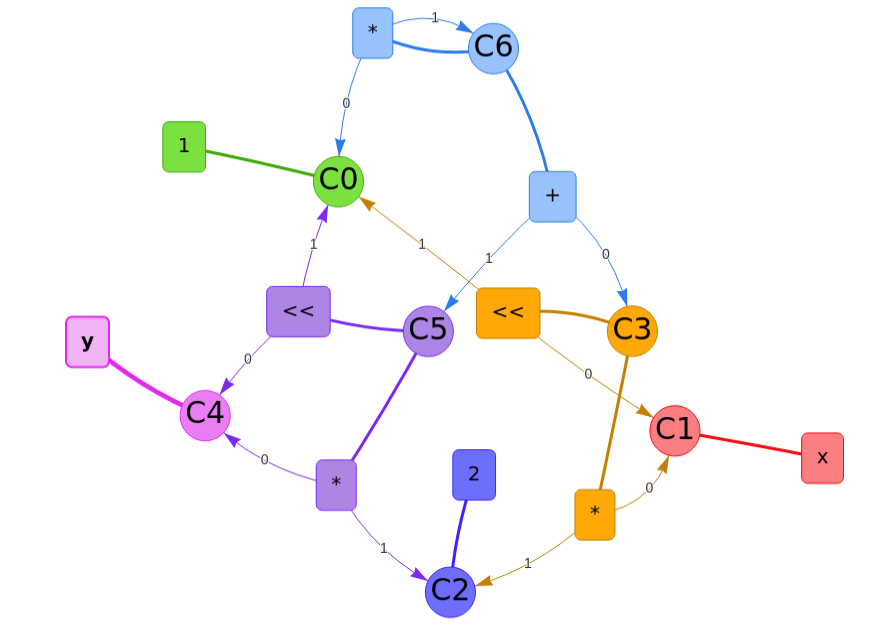
\includegraphics[width=1.2\columnwidth]{after-2.png}
    \caption{Graph from Figure \ref{fig:after_1} after applying the rewrite rule
      \texttt{(* pa 2) $\rightarrow$ (<< pa 1)}. }
    \label{fig:after_2}
\end{figure*}
\end{document}
